\chapter{Related Works}

Your related works, and your purpose and contribution which must be different as below.

\section{Same Topics}
Cite every latest journal with same topic
\subsection{Topic 1}
cite for first topic

\subsection{Topic 2}
if you have two topics you can include here to


\section{Same Method}
write and cite latest journal with same method

\subsection{Method 1}
cite and paraphrase method 1

\subsection{Method 2}
cite and paraphrase method 2 if you have more method please add new subsection.

\section{Yusniar Nur Syarif Sidiq/1164089}
\subsection{Binary Classification}
\begin{enumerate}
\item Binary Classification atau diartikan kedalam bahasa indonesia yaitu Klasifikasi Biner adalah tugas dalam mengkalrifikasikan elemen-elemen dari himpunan yang diberikan kedalam dua kelompok berdasarkan aturan klarifikasi. Pada ummnya klarifikasi biner akan jatuh ke dalam domain Supervised Learning dan dimana kasus khusus hanya memiliki dua kelas. Beberapa contoh yang meliputi Binary Classification adalah \begin{itemize}
		\item Deteksi Transaksi Penipuan Kartu Kredit
		\item Diagnosa medis
		\item Deteksi Spam
	\end{itemize}
\subitem Untuk contoh Binary Classification dapat dilihat pada gambar \ref{YNBC}
		\begin{figure}[ht]
		\centerline{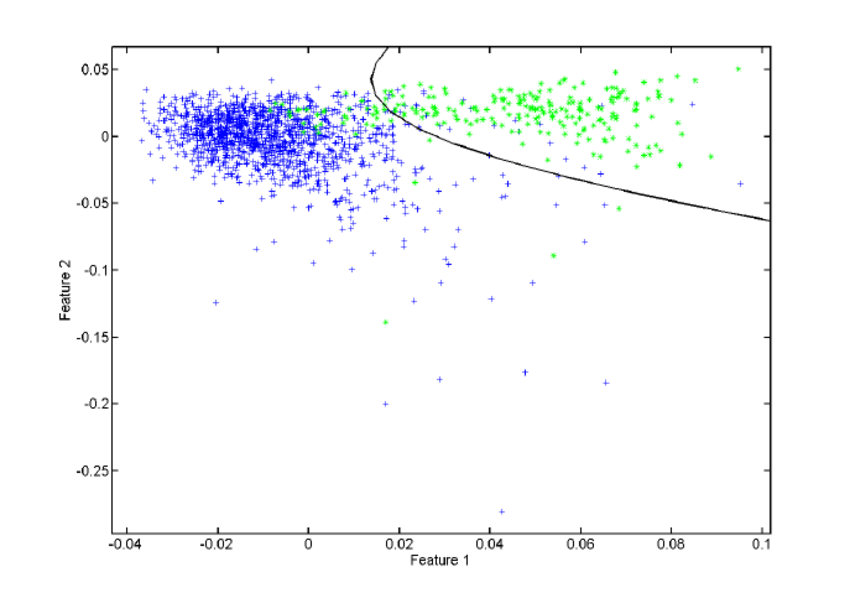
\includegraphics[width=1\textwidth]{figures/YN/YN50.png}}
		\caption{Binary Classification.}
		\label{YNBC}
		\end{figure}
 \end{enumerate}

\subsection{Supervised Learning, Unsupervised Learning, Dan Classtering}
\begin{enumerate}
\item Supervised Learning merupakan sebuah pendekatan yang dimana sudah adanya sdata yang dilatih dan telah terdapat variabel yang telah ditargetkan sehingga bertujuan untuk mengelompokkan suatu data ke data yang sudah ada. Contoh dalam Supervised Learning yaitu ketika anda memiliki sejumlah buku yang yang telah dilabel dengan urutan kategori tertentu. Ketika anda akan membeli sebuah buku baru, maka harus di identifikasi isi dari buku tersebut dan memasukkannya kedalam kategori tertentu. Ketika anda membeli sebuah buku tersebut maka anda telah menerapkan sebuah logika fuzzy. Ilustrasi Supervised Learning dapat dilihat pada gambar \ref{YNSL}.

		\begin{figure}[ht]
		\centerline{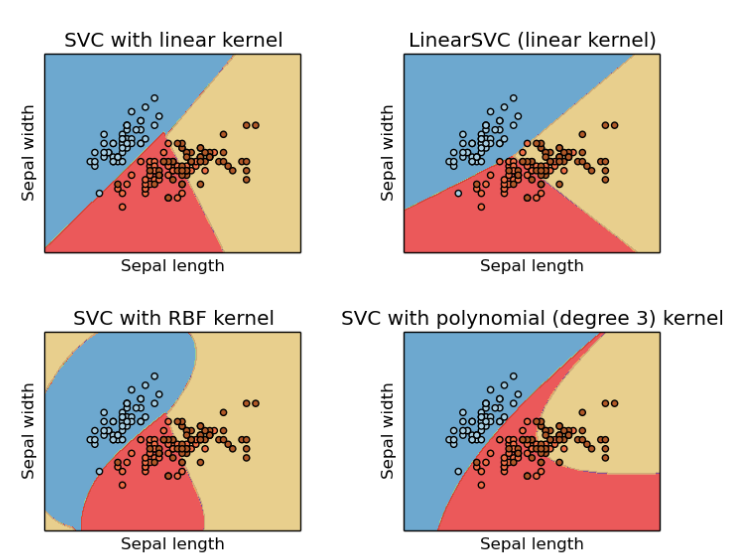
\includegraphics[width=1\textwidth]{figures/YN/YN51.png}}
		\caption{Supervised Learning.}
		\label{YNSL}
		\end{figure}

\item Unsupervised Learning merupakan sebuah data yang belum ditentukan variabelnya jadi hanya berupa data saja. Dalam sebuah kasus Unsupervised Learning adalah aggap saja anda belum pernah membeli buku sama sekali dan pada suatu hari anda telah membeli buku dengan sangat banyak dalam kategori yang berbeda. Sehingga buku tersebut belum di kategorikan dan hanya berupa data buku saja. Ilustrasi Unsupervised Learning dapat dilihat pada gambar \ref{YNUSL}.

		\begin{figure}[ht]
		\centerline{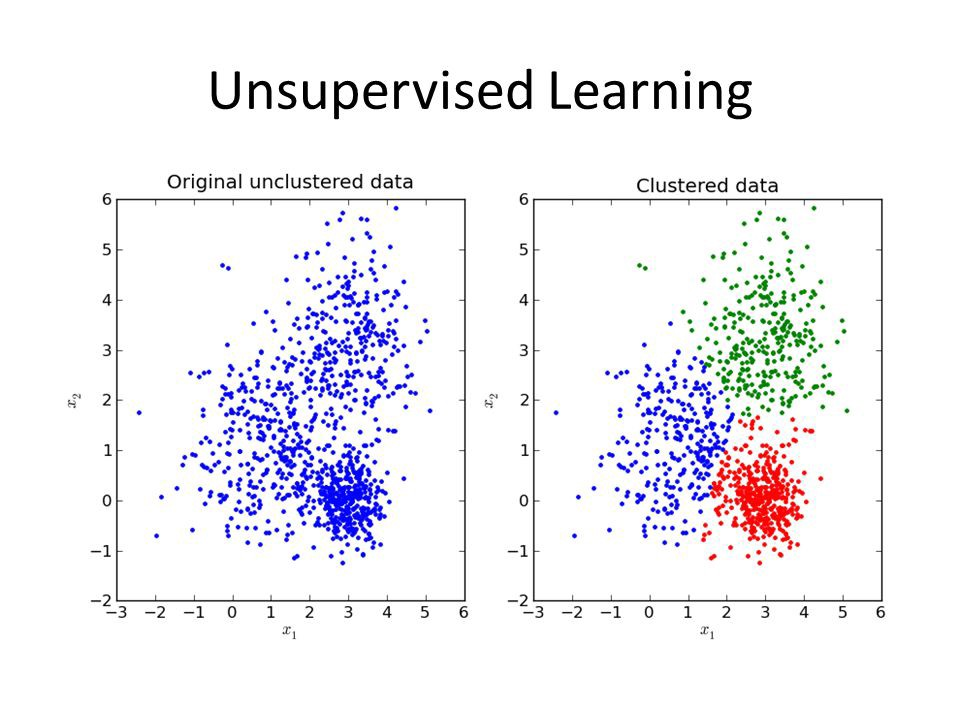
\includegraphics[width=1\textwidth]{figures/YN/YN52.jpeg}}
		\caption{Unsupervised Learning.}
		\label{YNUSL}
		\end{figure}

\item Classtering merupakan sebuah proses untuk mengklasifikasikan sebuah data dalam satu parameter. Dalam kasus ini dapat dijelaskan ada beberapa orang yang memiliki kekuatan tubuh yang sehat dan kekuatan tubuh yang lemah. Parameter bagi orang yang memiliki tubuh yang kuat adalah orang yang terlihat bugar dan sehat maka dengan orang yang memiliki parameter adalah orang yang memiliki kekuatan tubuh yang kuat dan untuk kekuatan tubuh yang lemah adalah sebaliknya. Ilustrasi gambar dapat di lihat di gambar \ref{YNC}

		\begin{figure}[ht]
		\centerline{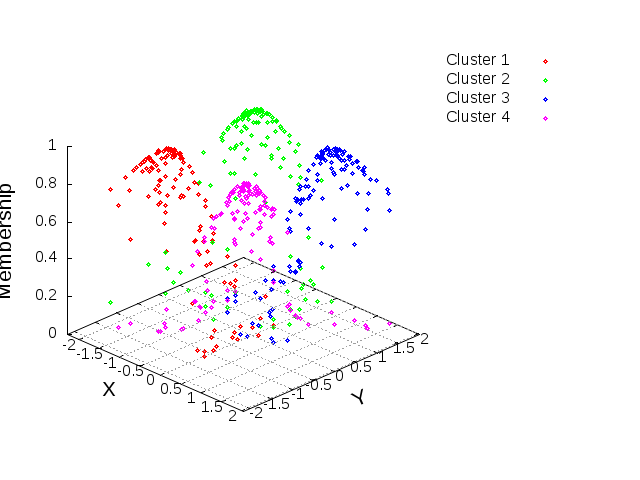
\includegraphics[width=1\textwidth]{figures/YN/YN53.png}}
		\caption{Clasterring.}
		\label{YNC}
		\end{figure}
\end{enumerate}

\subsection{Evaluasi Dan Akurasi}
\begin{enumerate}
\item Evaluasi dan akurasi adalah bagaimana cara kita dapat mengevaluasi sebarapa baik model melakukan pekerjaannya dengan cara mengukur akurasinya. Akurasi akan didefinisikan sebagai presentase kasus yang telah diklasifikasikan dengan benar. Kita dapat melakukan analisis kesalahan yang telah di buat oleh model.Dalam tabel tersebut baris true mangga dan true anggur menunjukkan kasus apakah itu objek mangga atau anggur. Kolom telah di prediksi dan dibuat oleh model. Ada 20 mangga yang di prediksi benar dan ada 5 anggur yang di prediksi salah. Ilustrasi dapat di lihat pada gambar \ref{YEA}

		\begin{figure}[ht]
		\centerline{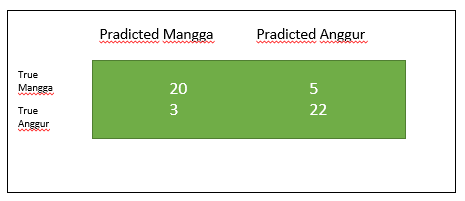
\includegraphics[width=1\textwidth]{figures/YN/YN54.png}}
		\caption{Evaluasi Dan Akurasi.}
		\label{YEA}
		\end{figure}
\end{enumerate}

\subsection{Confusion Matrix}
\begin{enumerate}
\item Ada beberapa cara untuk membuat dan membaca confusion matrix antara lain
	\begin{itemize}
		\item Tentukan pokok permasalahan serta atributnya
		\item Buat Decision Tree
		\item Buat Data Testing
		\item Mencari nilai variabelnya misal a,b,c, dan d
		\item Mencari nilai recall, precision, accuracy, dan erorr rate
	\end{itemize}
\subitem Di bawah ini adalah contoh dari confusion matrix
	\begin{verbatim}
		Recall =3/(1+3) = 0,75
		Precision = 3/(1+3) = 0,75
		Accuracy =(5+3)/(5+1+1+3) = 0,8
		Error Rate =(1+1)/(5+1+1+3) = 0,2 
	\end{verbatim}
\end{enumerate}

\subsection{Cara Kerja K-Fold Cross Validation}
\begin{enumerate}
\item Untuk cara kerja K-Fold Cross Validation adalah sebagai berikut
	\begin{itemize}
		\item Total instance dibagi menjadi N bagian.
		\item Fold yang pertama adalah bagian pertama menjadii testing data dan sisanya menjadi training data.
		\item Hitung akurasi berdasarkan porsi data tersebut dengan menggunakan persamaan.
		\item Fold yang ke dua adalah bagian ke dua menjadi testing data dan sisanya training data. 
		\item Hitung akurasi berdasarkan porsi data tersebut.
		\item Lakukan step secara berulang hingga habis mencapai fold ke-K.
		\item Terakhir hitung rata-rata akurasi K buah.
	\end{itemize}

\subitem Untuk ilustrasi K-Fold Cross Validation data di lihat pada gambar \ref{YNKF}
		\begin{figure}[ht]
		\centerline{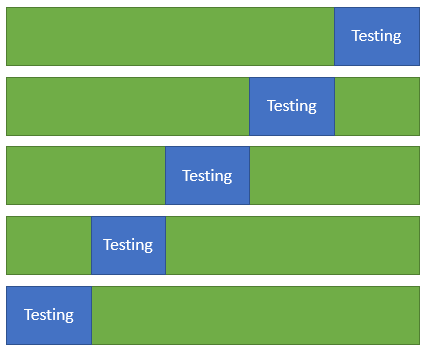
\includegraphics[width=1\textwidth]{figures/YN/YN55.png}}
		\caption{K-Fold Cross Validation.}
		\label{YNKF}
		\end{figure}
\end{enumerate}

\subsection{Decision Tree}
\begin{enumerate}
\item Decision Tree adalah sebuah metode pembelajaran yang digunakan untuk melakukan klarifikasi dan regresi. Decision Tree digunakan untuk membuat sebuah model yang dapat memprediksi sebuah nilai variabel target dengan cara mempelajari aturan keputusan dari fitur data. Contoh Decision Tree adalah untuk melakukan predikisi apakah Kuda termasuk hewan mamalia atau bukan, lihat pada gambar \ref{YNDT}.

		\begin{figure}[ht]
		\centerline{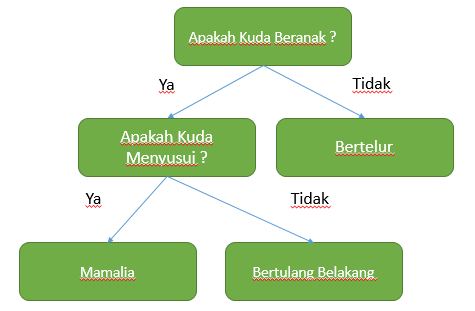
\includegraphics[width=1\textwidth]{figures/YN/YN56.png}}
		\caption{Decision Tree.}
		\label{YNDT}
		\end{figure}

\end{enumerate}

\subsection{Gain Dan Entropi}
\begin{enumerate}
\item Gain adalah pengurangan yang diharapkan dalam enthropy. Dalam mechine learning, gain dapat digunakan untuk menentukan sebuah urutan atribut atau memperkecil atribut yang telah dipilih. Urutan ini akan membentuk decision tree. atribut gain dipilih yang paling besar.

\item Entropi adalah ukuran ketidakpastian sebuah variabel acak sehingga dapat di artikan entropi adalah ukuran ketidakpastian dari sebuah atribut.

\subitem Ilustrasi dari gain dan entropi adalah bagaimana kita memprediksi jenis kelamin berdasarkan atributnya, perhatikan pada gambar \ref{YNGE}

		\begin{figure}[ht]
		\centerline{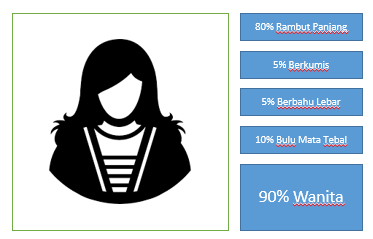
\includegraphics[width=1\textwidth]{figures/YN/YN57.png}}
		\caption{Gain Dan Entropi.}
		\label{YNGE}
		\end{figure}
\end{enumerate}

 \section{Andri Fajar Sunandhar/1164065}
\subsection{binary classification dilengkapi ilustrasi gambar}
\begin{enumerate}
\item Binary classification yaitu berupa kelas positif dan kelas negatif. Klasifikasi biner adalah dikotomisasi yang diterapkan untuk tujuan praktis, dan dalam banyak masalah klasifikasi biner praktis, kedua kelompok tidak simetris - daripada akurasi keseluruhan, proporsi relatif dari berbagai jenis kesalahan yang menarik. Misalnya, dalam pengujian medis, false positive (mendeteksi penyakit ketika tidak ada) dianggap berbeda dari false negative (tidak mendeteksi penyakit ketika hadir).
\begin{figure}[ht]
\centering
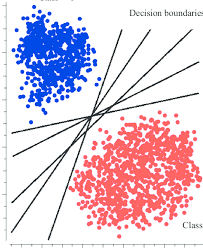
\includegraphics[scale=0.5]{figures/AFS/andri1.png}
\caption{Binary Classification}
\label{contoh}
\end{figure}
\end{enumerate}

\subsection{supervised learning dan unsupervised learning dan clustering dengan ilustrasi gambar}
\begin{enumerate}
\item Supervised learning adalah tugas pembelajaran mesin untuk mempelajari suatu fungsi yang memetakan input ke output berdasarkan contoh pasangan input-output. Ini menyimpulkan fungsi dari data pelatihan berlabel yang terdiri dari serangkaian contoh pelatihan. Dalam pembelajaran yang diawasi, setiap contoh adalah pasangan yang terdiri dari objek input (biasanya vektor) dan nilai output yang diinginkan (juga disebut sinyal pengawas). Algoritma pembelajaran yang diawasi menganalisis data pelatihan dan menghasilkan fungsi yang disimpulkan, yang dapat digunakan untuk memetakan contoh-contoh baru. Skenario optimal akan memungkinkan algoritma menentukan label kelas dengan benar untuk instance yang tidak terlihat. Ini membutuhkan algoritma pembelajaran untuk menggeneralisasi dari data pelatihan untuk situasi yang tidak terlihat dengan cara yang "masuk akal" (lihat bias induktif). Tugas paralel dalam psikologi manusia dan hewan sering disebut sebagai pembelajaran konsep. Contoh dibawah yaitu Supervised Learning dengan SVC.
\begin{figure}[ht]
\centering
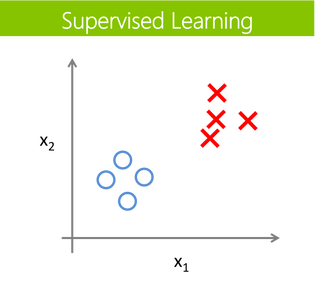
\includegraphics[scale=0.5]{figures/AFS/andri2.png}
\caption{Supervised Learning}
\label{contoh}
\end{figure}
\item Unsupervised learning adalah istilah yang digunakan untuk pembelajaran bahasa Ibrani, yang terkait dengan pembelajaran tanpa guru, juga dikenal sebagai organisasi mandiri dan metode pemodelan kepadatan probabilitas input. Analisis cluster sebagai cabang pembelajaran mesin yang mengelompokkan data yang belum diberi label, diklasifikasikan atau dikategorikan. Alih-alih menanggapi umpan balik, analisis klaster mengidentifikasi kesamaan dalam data dan bereaksi berdasarkan ada tidaknya kesamaan di setiap potongan data baru. BErikut merupakan contoh Unsupervised Learning dengan Gaussian mixture models.
\begin{figure}[ht]
\centering
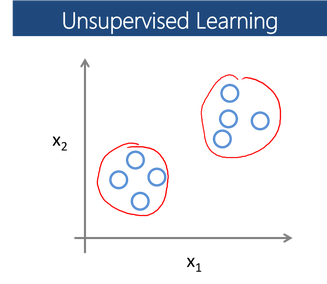
\includegraphics[scale=0.5]{figures/AFS/andri3.png}
\caption{Unsupervised Learning}
\label{contoh}
\end{figure}
\item Cluster analysis or clustering adalah tugas pengelompokan sekumpulan objek sedemikian rupa sehingga objek dalam kelompok yang sama (disebut klaster) lebih mirip (dalam beberapa hal) satu sama lain daripada pada kelompok lain (kluster). Ini adalah tugas utama penambangan data eksplorasi, dan teknik umum untuk analisis data statistik, yang digunakan di banyak bidang, termasuk pembelajaran mesin, pengenalan pola, analisis gambar, pengambilan informasi, bioinformatika, kompresi data, dan grafik komputer. Analisis Cluster sendiri bukan merupakan salah satu algoritma spesifik, tetapi tugas umum yang harus dipecahkan. Ini dapat dicapai dengan berbagai algoritma yang berbeda secara signifikan dalam pemahaman mereka tentang apa yang merupakan sebuah cluster dan bagaimana cara menemukannya secara efisien. Gagasan populer mengenai cluster termasuk kelompok dengan jarak kecil antara anggota cluster, area padat ruang data, interval atau distribusi statistik tertentu. Clustering karena itu dapat dirumuskan sebagai masalah optimasi multi-objektif. Algoritma pengelompokan dan pengaturan parameter yang sesuai (termasuk parameter seperti fungsi jarak yang akan digunakan, ambang kepadatan atau jumlah cluster yang diharapkan) tergantung pada set data individual dan penggunaan hasil yang dimaksudkan. Analisis kluster bukan merupakan tugas otomatis, tetapi proses berulang penemuan pengetahuan atau optimasi multi-objektif interaktif yang melibatkan percobaan dan kegagalan. Seringkali diperlukan untuk memodifikasi praproses data dan parameter model hingga hasilnya mencapai properti yang diinginkan.
\begin{figure}[ht]
\centering
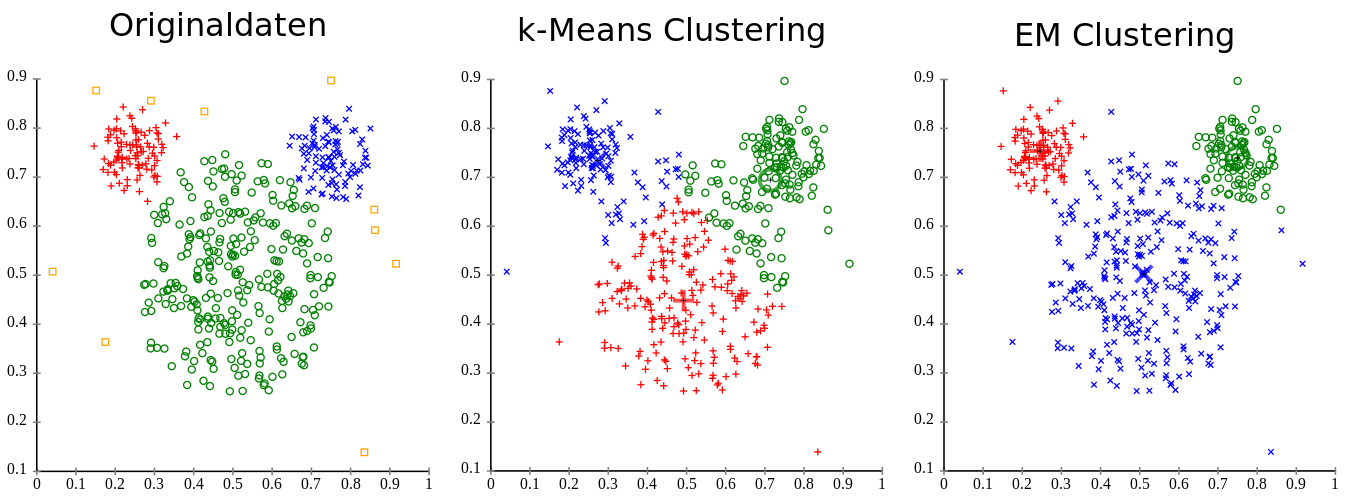
\includegraphics[scale=0.5]{figures/AFS/andri4.png}
\caption{Cluster}
\label{contoh}
\end{figure}
\end{enumerate}

\subsection{evaluasi dan akurasi dari buku dan disertai ilustrasi contoh
dengan gambar}
\begin{enumerate}
\item Evaluasi adalah tentang  bagaimana kita dapat mengevaluasi seberapa baik model bekerja dengan mengukur akurasinya. Dan akurasi akan didefinisikan sebagai persentase kasus yang diklasifikasikan dengan benar. Kita dapat menganalisis kesalahan yang dibuat oleh model, atau tingkat kebingungannya, menggunakan matriks kebingungan. Matriks kebingungan mengacu pada kebingungan dalam model, tetapi matriks kebingungan ini bisa menjadi sedikit sulit untuk dipahami ketika mereka menjadi sangat besar.
\begin{figure}[ht]
\centering
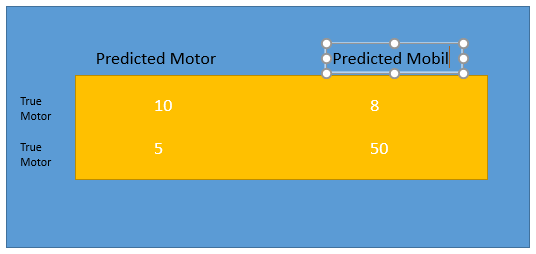
\includegraphics[scale=0.5]{figures/AFS/andri5.png}
\caption{ Evaluasi dan Akurasi}
\label{contoh}
\end{figure}
\end{enumerate}

\subsection{ bagaimana cara membuat dan membaca confusion matrix, buat confusion matrix }
\begin{enumerate}
\item Cara membuat dan membaca confusion matrix :
\begin{itemize}
\item 1)	Tentukan pokok permasalahan dan atributanya, misal gaji dan listik.
\item 2)	Buat pohon keputusan
\item 3)	Lalu data testingnya
\item 4)	Lalu mencari nilai a, b, c, dan d. Semisal a = 5, b = 1, c = 1, dan d = 3.
\item 5)	Selanjutnya mencari nilai recall, precision, accuracy, serta dan error rate.
\end{itemize}
\item Berikut adalah contoh dari confusion matrix :
\begin{itemize}
\item Recall =3/(1+3) = 0,75
\item Precision = 3/(1+3) = 0,75
\item Accuracy =(5+3)/(5+1+1+3) = 0,8
\item Error Rate =(1+1)/(5+1+1+3) = 0,2
\end{itemize}
\end{enumerate}

\subsection{bagaimana K-fold cross validation bekerja dengan gambar ilustrasi}
\begin{enumerate}
\item Cara kerja K-fold cross validation :
\begin{itemize}
\item 1)	Total instance dibagi menjadi N bagian.
\item 2)	Fold yang pertama adalah bagian pertama menjadi data uji (testing data) dan sisanya menjadi training data.
\item 3)	Lalu hitung akurasi berdasarkan porsi data tersebut dengan menggunakan persamaan.
\item 4)	Fold yang ke dua adalah bagian ke dua menjadi data uji (testing data) dan sisanya training data. 
\item 5)	Kemudian hitung akurasi berdasarkan porsi data tersebut.
\item 6)	Dan seterusnya hingga habis mencapai fold ke-K.
\item 7)	Terakhir hitung rata-rata akurasi K buah.
\end{itemize}
\begin{figure}[ht]
\centering
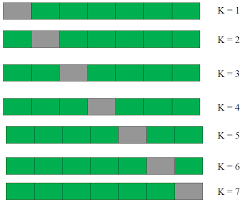
\includegraphics[scale=0.5]{figures/AFS/andri6.png}
\caption{K-fold cross validation }
\label{contoh}
\end{figure}
\end{enumerate}

\subsection{decision tree dengan gambar ilustrasi}
\begin{enumerate}
\item Decision Tree dalah metode pembelajaran yang diawasi non-parametrik yang digunakan untuk klasifikasi dan regresi. Tujuannya adalah untuk membuat model yang memprediksi nilai variabel target dengan mempelajari aturan keputusan sederhana yang disimpulkan dari fitur data.\\
Misalnya, dalam contoh di bawah ini, decision tree belajar dari data untuk memperkirakan kurva sinus dengan seperangkat aturan keputusan if-then-else. Semakin dalam pohon, semakin rumit aturan keputusan dan semakin bugar modelnya.
\begin{figure}[ht]
\centering
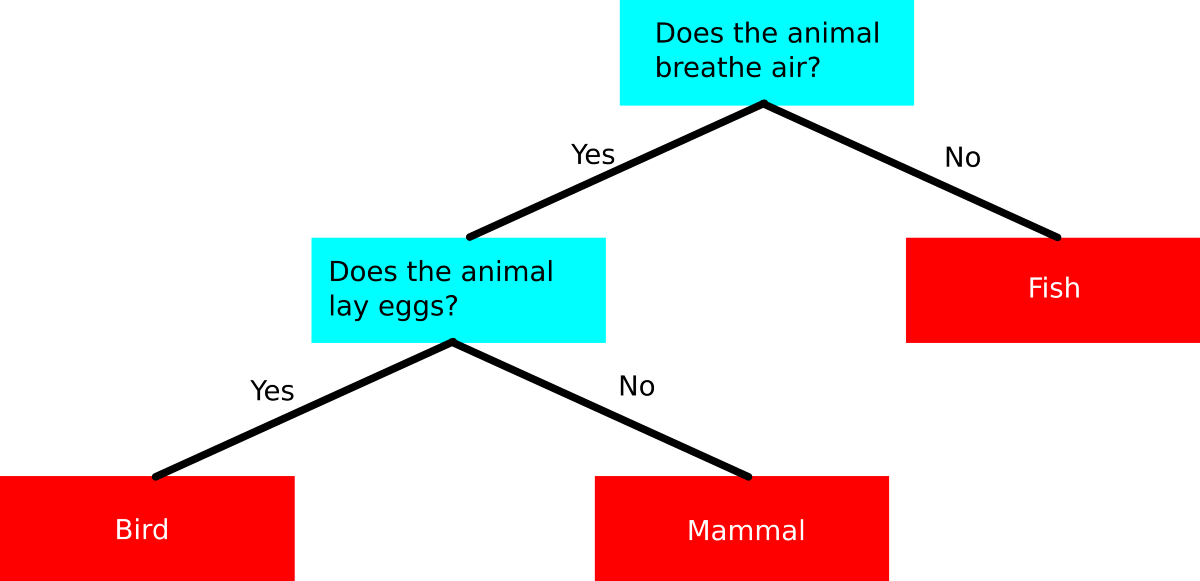
\includegraphics[scale=0.5]{figures/AFS/andri7.png}
\caption{Decision Tree}
\label{contoh}
\end{figure}
\end{enumerate}

\subsection{Information Gain dan entropi dengan gambar ilustrasi}
\begin{enumerate}
\item Information gain didasarkan pada penurunan entropi setelah dataset dibagi pada atribut. Membangun decision tree adalah semua tentang menemukan atribut yang mengembalikan perolehan informasi tertinggi (mis., Cabang yang paling homogen).
\begin{figure}[ht]
\centering

\includegraphics[scale=0.5]{figures/AFS/andri8.png}
\caption{Information gain}
\label{contoh}
\end{figure}
\item Entropi adalah ukuran keacakan dalam informasi yang sedang diproses. Semakin tinggi entropi, semakin sulit untuk menarik kesimpulan dari informasi itu. Membalik koin adalah contoh tindakan yang memberikan informasi yang acak. Untuk koin yang tidak memiliki afinitas untuk kepala atau ekor, hasil dari sejumlah lemparan sulit diprediksi. Mengapa? Karena tidak ada hubungan antara membalik dan hasilnya. Inilah inti dari entropi.
\end{enumerate}

\section{Imron Sumadireja / 1164076}
\subsection{Binary Classification}
\begin{enumerate}
\item Binary classification merupakan suatu cara untuk mengklasifikasikan atau mengkategorikan objek set dengan atribut ke dalam ke dua kategori yang sudah ada atau biasa di sebut dengan supervised. Binary classification dapat diterapkan dengan tujuan praktis, dalam banyak masalah binary classification. Untuk contoh binary classification dapat dilihat pada gambar \ref{bc}
		\begin{figure}[ht]
		\centerline{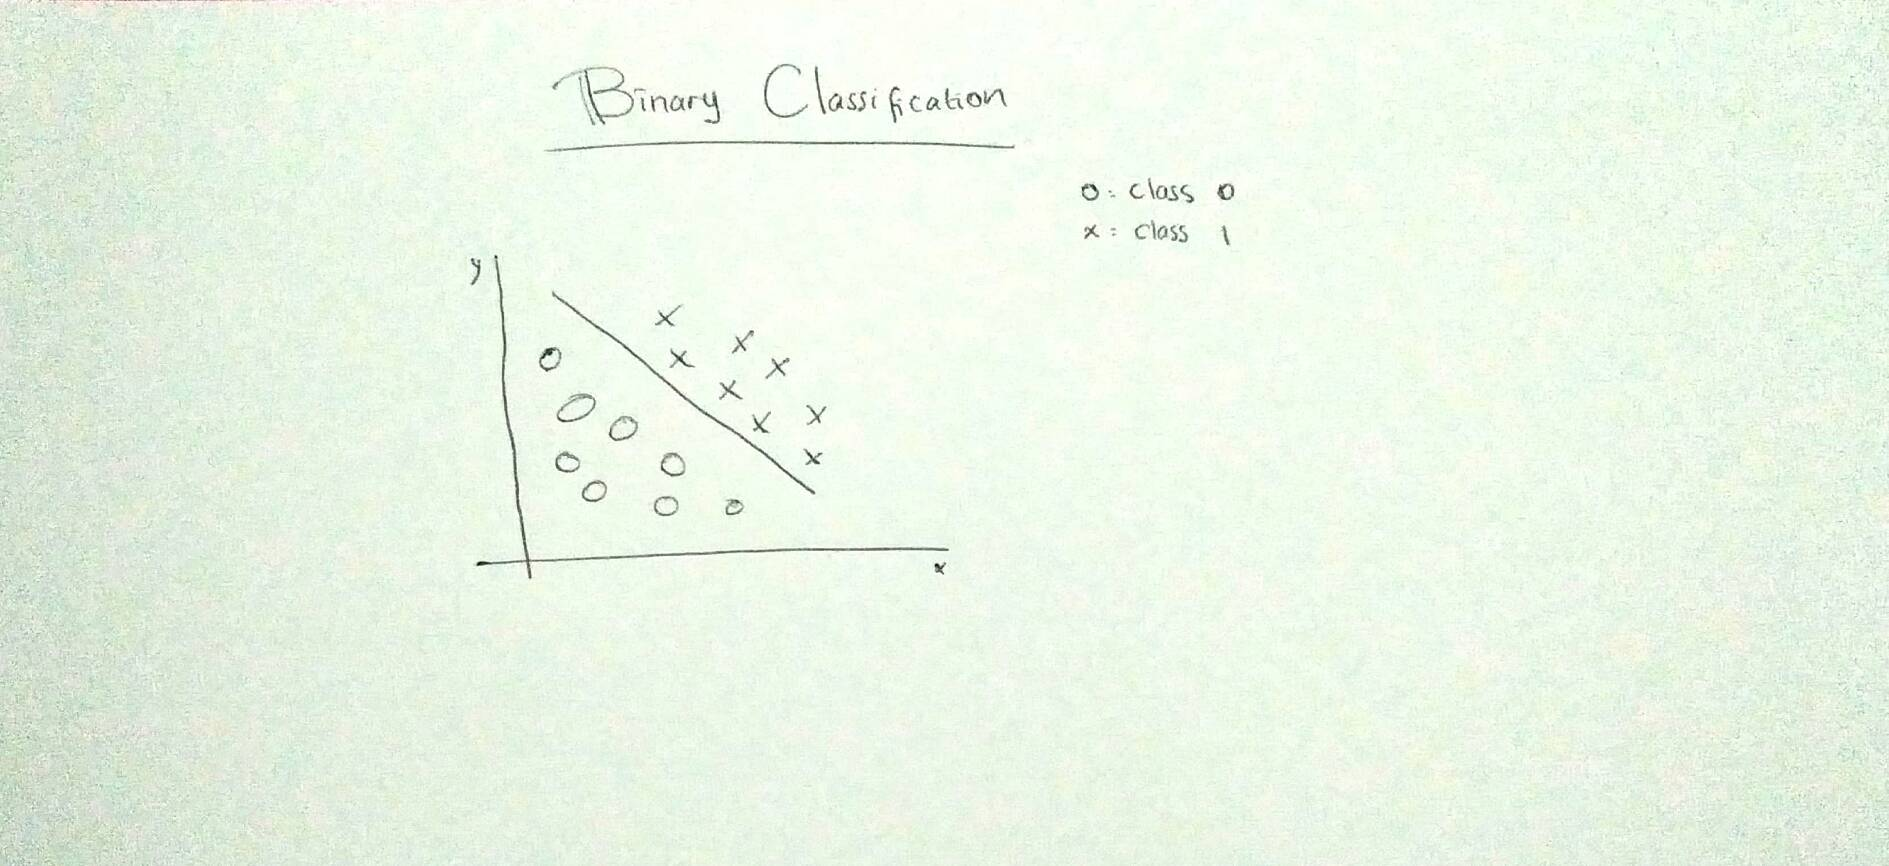
\includegraphics[width=1\textwidth]{figures/im/im11.jpg}}
		\caption{Binary Classification.}
		\label{bc}
		\end{figure}
\end{enumerate}

\subsection{Supervised Learning, Unsupervised Learning, dan Classtering}
\begin{enumerate}
\item Supervised learning merupakan suatu pembelajaran bagi mesin untuk mempelajari suatu fungsi yang memetakan input ke output berdasarkan data yang telah diberikan dan terdapat variable yang telah ditargetkan sehingga tujuan dari pembelajaran ini mesin dapat memetakan output dengan baik. Sehingga proses training yang dilakukan pada mesin dapat berjalan sesuai dengan target yang ditentukan dan hasil dari data training tersebut dapat digunakan untuk melakukan prediksi.Contoh supervised learning dapat dilihat pada gambar berikut \ref{sl}
		\begin{figure}[ht]
		\centerline{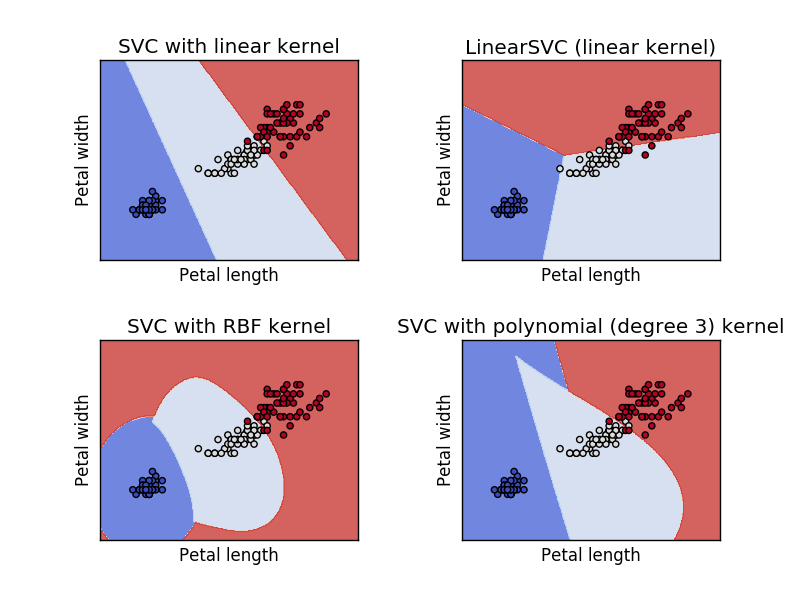
\includegraphics[width=1\textwidth]{figures/im/im22.png}}
		\caption{Supervised Learning.}
		\label{sl}
		\end{figure}

\item Unsupervised learning merupakan suatu pembelajaran bagi mesin, namun tidak memiliki data latih, atau data training. Unsupervised ini dapat mengklasifikasikan suatu objek secara langsung dengan atribut seadanya pada data tersebut. Sebagai contoh, jika kita ingin mengelompokkan sekumpulan orang hanya diperlukan dari data yang ada misalnya dari jenis kelamin, pakaian yang digunakan, dan lain sebagainya. Oleh karena itu unsupervised learning ini tidak memiliki data training. Contoh supervised learning dapat dilihat pada gambar berikut \ref{ul}
		\begin{figure}[ht]
		\centerline{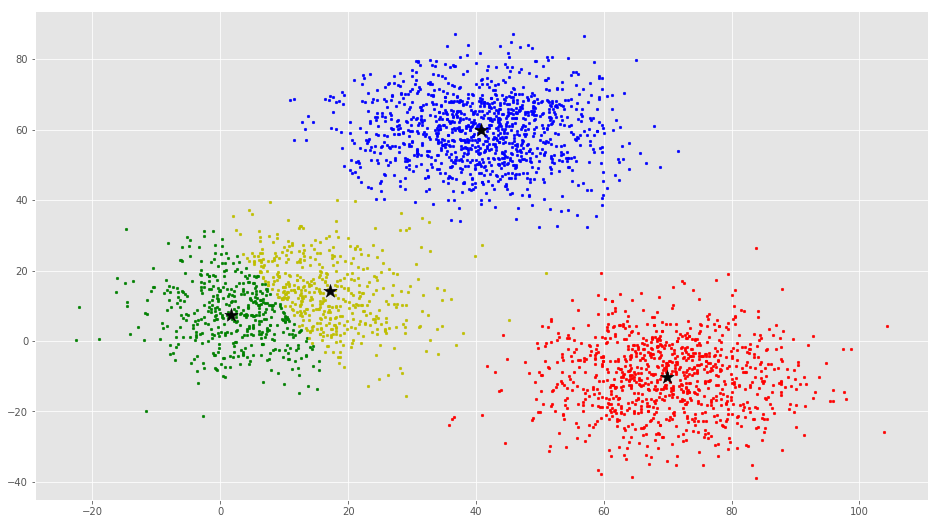
\includegraphics[width=1\textwidth]{figures/im/im33.png}}
		\caption{Unsupervised Learning.}
		\label{ul}
		\end{figure}

\item Clustering adalah metode pengelompokan data ke dalam beberapa cluster atau kelompok agar data dalam satu cluster tersebut memiliki tingkat kemiripan yang maksimum dan data dengan kemiripan yang minimum. Clustering merupakan proses satu set data ke dalam himpunan bagian atau kelompok yang disebut dengan cluster. Contoh clustering dapat dilihat pada gambar berikut \ref{c}
		\begin{figure}[ht]
		\centerline{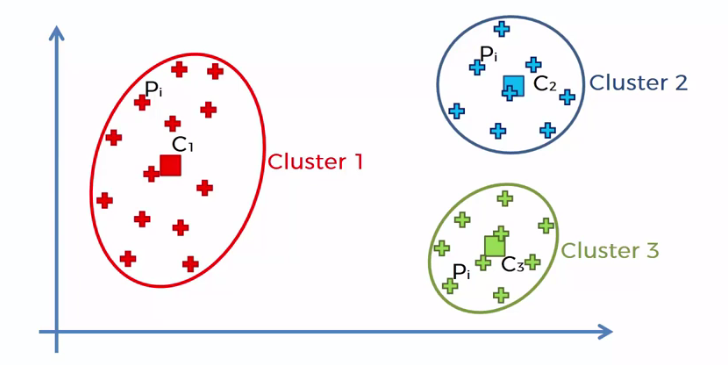
\includegraphics[width=1\textwidth]{figures/im/im44.png}}
		\caption{Clustering.}
		\label{c}
		\end{figure}
\end{enumerate}

\subsection{Evaluasi dan Akurasi}
\begin{enumerate}
\item Evaluasi adalah tentang bagaimana dapat mengevaluasi seberapa baik model bekerja dengan mengukur akurasinya. Dan akurasi akan didefinisikan sebagai persentase kasus yang diklasifikasikan dengan benar. Kita dapat menganalisis kesalahan yang dibuat oleh model, atau tingkat kebingungannya, menggunakan matriks kebungungan. Matriks kebingungan mengacu pada kebingungan mengacu pada kebingungan dalam model, tetapi matriks kebingungan ini bisa menjadi sedikit lebih sulit untuk dipahami ketika mereka menjadi sangat besar. Contohnya dapat dilihat pada gambar berikut \ref{EA}
		\begin{figure}[ht]
		\centerline{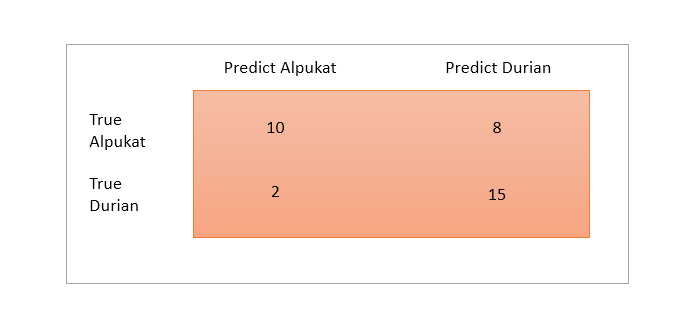
\includegraphics[width=1\textwidth]{figures/im/im00.png}}
		\caption{Evaluasi dan Akurasi.}
		\label{c}
		\end{figure}
\end{enumerate}

\subsection{Confusion Matrix}
\begin{enumerate}
\item Terdapat beberapa cara untuk membuat dan membaca confusion matrix diantaranya, sebagai berikut
	\begin{itemize}
		\item Tentukan pokok permasalahan dan atributnya, misal pendapatan dan pengeluaran.
		\item Buat decission tree
		\item Buat data testingnya
		\item Lalu mencari nilai a, b ,c dan d. Misal a = 8, b = 2, c = 2, dan d = 6.
		\item Selanjutnya mencari nilai recall, precision, accuracy, dan error rate.
	\end{itemize}
\subitem Berikut contoh dari confusion matrix
	\begin{verbatim}
		Recall = 6/(2+6) = 1,33
		Precision = 6/(2+6) = 1,33
		Accuracy = (8+6)/(8+2+2+6) = 0,8
		Error rate = (2+2)/(8+2+2+6) = 0,22
	\end{verbatim}
\end{enumerate}

\subsection{Cara kerja K-Fold Cross Validation}
\begin{enumerate}
\item Untuk cara kerja K-Fold Cross Validation sebagai berikut
	\begin{itemize}
		\item Total instance dibagi menjadi N bagian
		\item Fold yang pertama adalah bagian pertama menjadi data uji (testing) dan sisanya menjadi training data
		\item Lalu hitung akurasi berdasarkan porsi data tersebut dengan menggunakan persamaan
		\item Fold yang kedua adalah bagian ke dua menjadi data uji (testing) dan sisanya menjadi training data
		\item Lalu hitung akurasi berdasarkan porsi data tersebut
		\item Dan selanjutnya hingga mencapai fold ke-4
		\item Terakhir hitung rata-rata akurasi K buah.
	\end{itemize}
\subitem Ilustrasi dari K-Fold Cross Validation dapat dilihat pada gambar \ref{KF}
		\begin{figure}[ht]
		\centerline{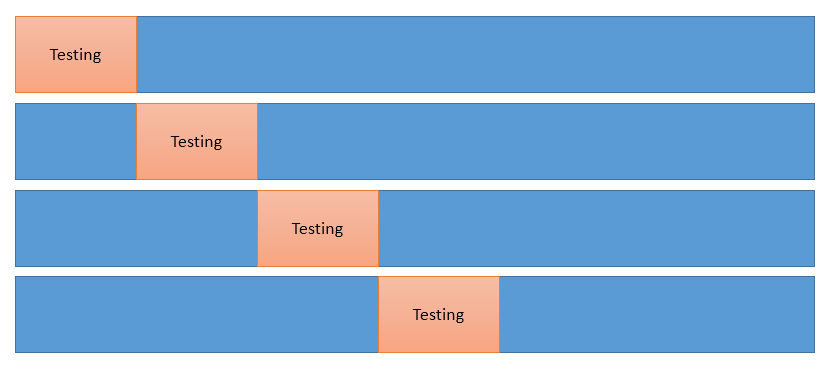
\includegraphics[width=1\textwidth]{figures/im/im55.png}}
		\caption{K-Fold Cross Validation.}
		\label{KF}
		\end{figure}
\end{enumerate}

\subsection{Decision Tree}
\begin{enumerate}
\item Decision tree adalah sebuah metode pembelajaran yang diawasi non-parametik digunakan untuk klasifikasi dan regresi. Decision tree digunakan untuk membuat sebuah model yang dapat memprediksi variable dengan mempelajari aturan keputusan dengan ciri-ciri yang terdapat pada atribut tersebut. Sebagai contoh decision tree dapat melakukan prediksi apakah di bulan terdapat gravitasi atau bukan. Contohnya dapat dilihat pada gambar berikut \ref{DT}
		\begin{figure}[ht]
		\centerline{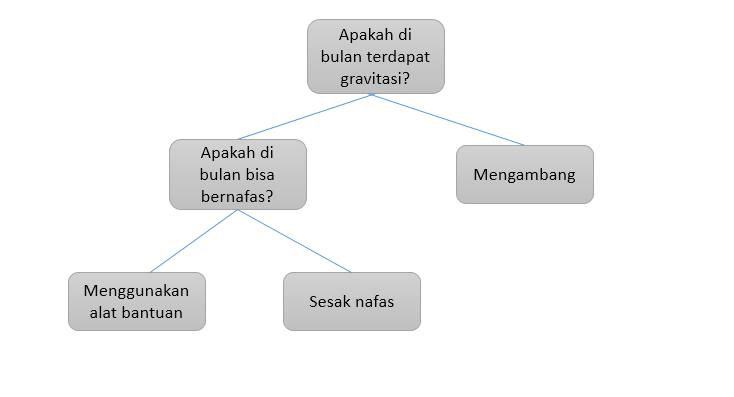
\includegraphics[width=1\textwidth]{figures/im/im66.png}}
		\caption{Decision Tree.}
		\label{DT}
		\end{figure}
\end{enumerate}

\subsection{Information Gain dan Entropi}
\begin{enumerate}
\item Information Gain adalah informasi atau kriteria dalam pembagian sebuah objek. Sebagai contoh misalnya information gain pada gambar laki-laki, atribut yang biasanya dimiliki pada gambar laki-laki diantaranya berambut pendek, berjakun, berjenggot, berkumis. Dalam beberapa hal terdapat perempuan yang memiliki rambut pendek, berkumis, dan berjenggot, namun dari parameter yang telah di identifikasi bahwa gambar tersebut memiliki akurasi yang lebih tinggi jadi dapat disimpulkan bahwa gambar tersebut adalah laki-laki. Untuk lebih jelasnya bisa dilihat dalam gambar \ref{IGE}

\item Entropi merupakan ukuran dari keacakan informasi, semakin tinggi entropi maka akan semakin sulit dalam menentukan suatu keputusan
		\begin{figure}[ht]
		\centerline{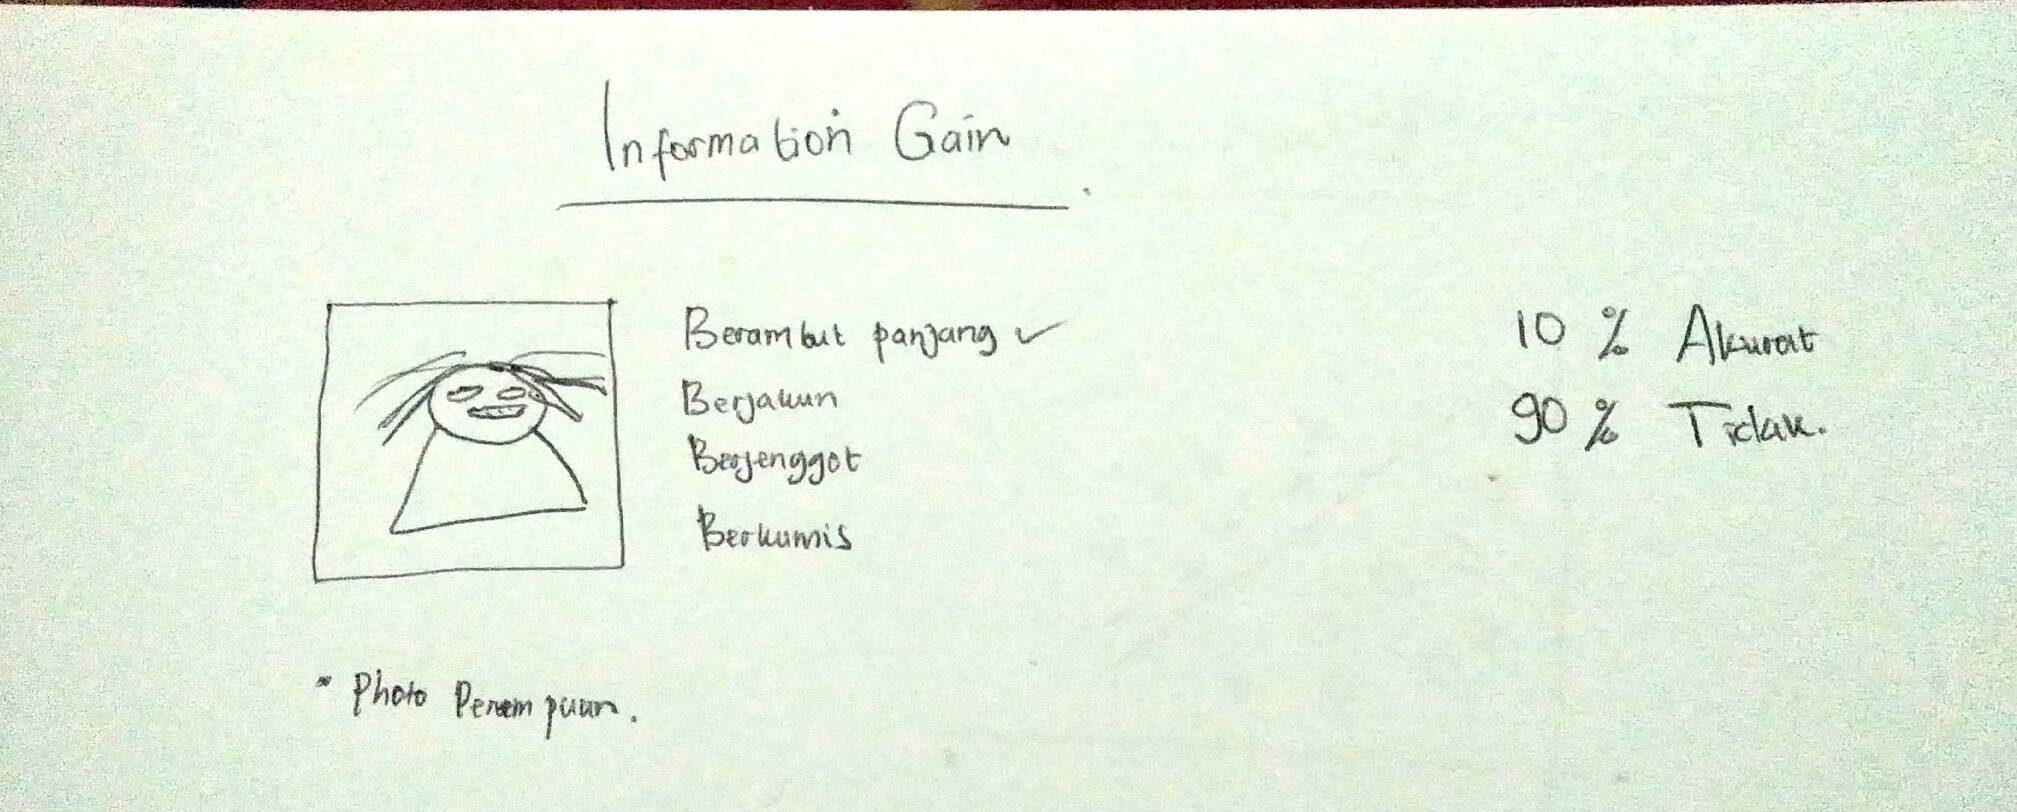
\includegraphics[width=1\textwidth]{figures/im/im77.jpg}}
		\caption{Information Gain dan Entropi.}
		\label{IGE}
		\end{figure}
\end{enumerate}

\section{Imron Sumadireja / 1164076}
\subsection{scikit-learn}
Pada praktikum kali ini saya merubah beberapa variable yang terdapat pada source code dengan nama kota.
Source code 1:
		\begin{figure}[ht]
		\centerline{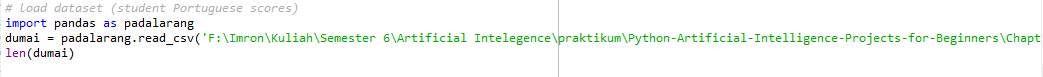
\includegraphics[width=1\textwidth]{figures/im/imQ1.png}}
		\caption{Source Code.}
		\label{satuQ}
		\end{figure}
\begin{itemize}
\item Pada baris pertama dari source code tersebut menjelaskan bahwa kita akan import library pandas dengan merubah nama alias menjadi padalarang, seperti gambar berikut \ref{satuQ}
\item Pada baris kedua terdapat variable baru dengan nama dumai, dan akan membaca file dengan ekstensi .csv
\item Berikut hasil yang di dapat dari source code berikut \ref{satuC}
		\begin{figure}[ht]
		\centerline{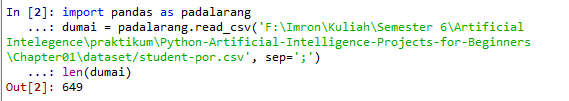
\includegraphics[width=1\textwidth]{figures/im/imCode1.png}}
		\caption{Source Code.}
		\label{satuC}
		\end{figure}
\end{itemize}

Source code 2:
		\begin{figure}[ht]
		\centerline{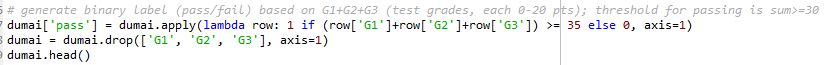
\includegraphics[width=1\textwidth]{figures/im/imQ2.png}}
		\caption{Source Code.}
		\label{duaQ}
		\end{figure}
\begin{itemize}
\item Pada baris pertama menjelaskan bahwa kita akan menambahkan kolom lulus atau gagal. Data dari kolom tersebut akan berisi 1 dan 0. 1 Untuk mahasiswa yang dinyatakan lulus dan 0 untuk mahasiswa yang tidak lulus, seperti gambar berikut \ref{duaQ}
\item Pada baris kedua akan membuat data-data tersebut disusun secara berurutan sesuai atribut
\item Pada baris ketiga berguna untuk menyinkronkan data yang terdapat pada source code pertama
\item Berikut hasil yang di dapat dari source code berikut \ref{duaC}
		\begin{figure}[ht]
		\centerline{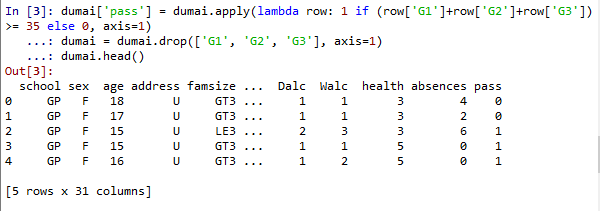
\includegraphics[width=1\textwidth]{figures/im/imCode2.png}}
		\caption{Source Code.}
		\label{duaC}
		\end{figure}
\end{itemize}

Source code 3:
		\begin{figure}[ht]
		\centerline{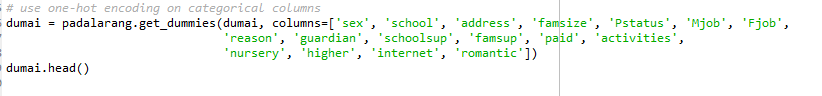
\includegraphics[width=1\textwidth]{figures/im/imQ3.png}}
		\caption{Source Code.}
		\label{tigaQ}
		\end{figure}
\begin{itemize}
\item Pada baris pertama menjelaskan bahwa dalam data tersebut akan memberikan tambahan kolom dengan atribut dengan isi 0 dan 1, seperti gambar berikut \ref{tigaQ}
\item Pada baris kedua berguna untuk menyinkronkan data yang terdapat pada source code sebelumnya
\item Berikut hasil yang di dapat dari source code berikut \ref{tigaC}
		\begin{figure}[ht]
		\centerline{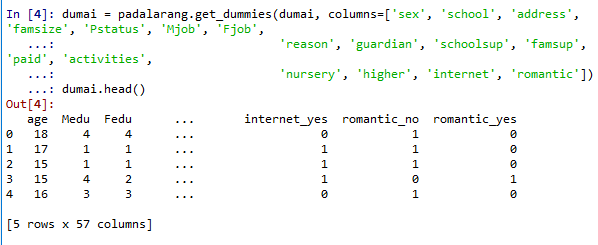
\includegraphics[width=1\textwidth]{figures/im/imCode3.png}}
		\caption{Source Code.}
		\label{tigaC}
		\end{figure}
\end{itemize}

Source code 4:
		\begin{figure}[ht]
		\centerline{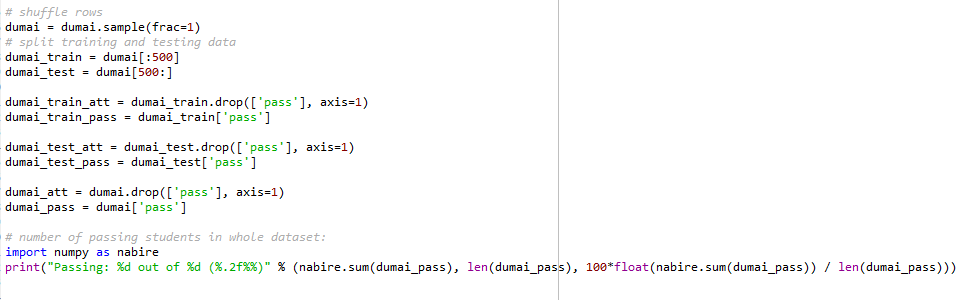
\includegraphics[width=1\textwidth]{figures/im/imQ4.png}}
		\caption{Source Code.}
		\label{empatQ}
		\end{figure}
\begin{itemize}
\item Pada baris pertama menjelaskan bahwa variable dumai akan menjalankan fungsi sample dengan frac 1, seperti gambar berikut \ref{empatQ}
\item Pada baris kedua dan ketiga berguna untuk memberikan data training dan data testing dengan masing-masing nilai 500
\item Pada baris keempat dan kelima berguna untuk melatih data training
\item Pada baris keenam dan ketujuh berguna untuk melatih data testing
\item Pada baris kedelapan dan kesembilan bergunan untuk membuat sebuah keputusan dari hasil data training dan data testing
\item Pada baris kesepuluh berguna untuk import library numpy
\item Pada baris kesebelas berguna untuk menampilkan hasil data suatu keputusan tersebut
\item Berikut hasil yang di dapat dari source cede berikut \ref{empatC}
		\begin{figure}[ht]
		\centerline{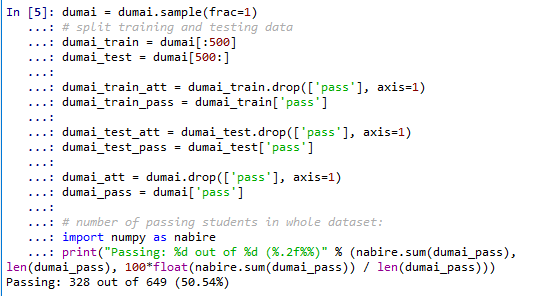
\includegraphics[width=1\textwidth]{figures/im/imCode4.png}}
		\caption{Source Code.}
		\label{empatC}
		\end{figure}
\end{itemize}

Source code 5:
		\begin{figure}[ht]
		\centerline{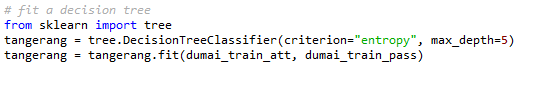
\includegraphics[width=1\textwidth]{figures/im/imQ5.png}}
		\caption{Source Code.}
		\label{limaQ}
		\end{figure}
\begin{itemize}
\item Pada baris pertama berguna untuk import libray tree yang berguna untuk membuat keputusan dengan metode tree, seperti gambar berikut \ref{limaQ}
\item Pada baris kedua variable tangerang akan menjalankan fungsi tree decision
\item Pada baris ketiga variable tangerang akan menjalankan fungsi tersebut menggunakan data training
\item Berikut hasil yang di dapat dari source code berikut \ref{limaC}
		\begin{figure}[ht]
		\centerline{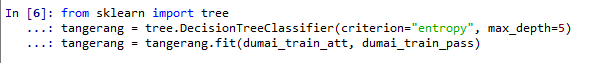
\includegraphics[width=1\textwidth]{figures/im/imCode5.png}}
		\caption{Source Code.}
		\label{limaC}
		\end{figure}
\end{itemize}

Source code 6:
		\begin{figure}[ht]
		\centerline{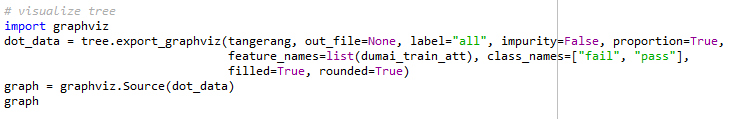
\includegraphics[width=1\textwidth]{figures/im/imQ6.png}}
		\caption{Source Code.}
		\label{enamQ}
		\end{figure}
\begin{itemize}
\item Pada baris pertama berguna untuk import library graphviz, seperti pada gambar berikut \ref{enamQ}
\item Pada baris kedua berguna untuk membuat graphviz dari hasil data yang telah di latih pada source code sebelumnya
\item Baris ketiga berguna untuk memanggil atribut dot untuk ditampilkan dalam bentuk graphic
\item Berikut hasil yang di dapat dari source code berikut \ref{enamC}
		\begin{figure}[ht]
		\centerline{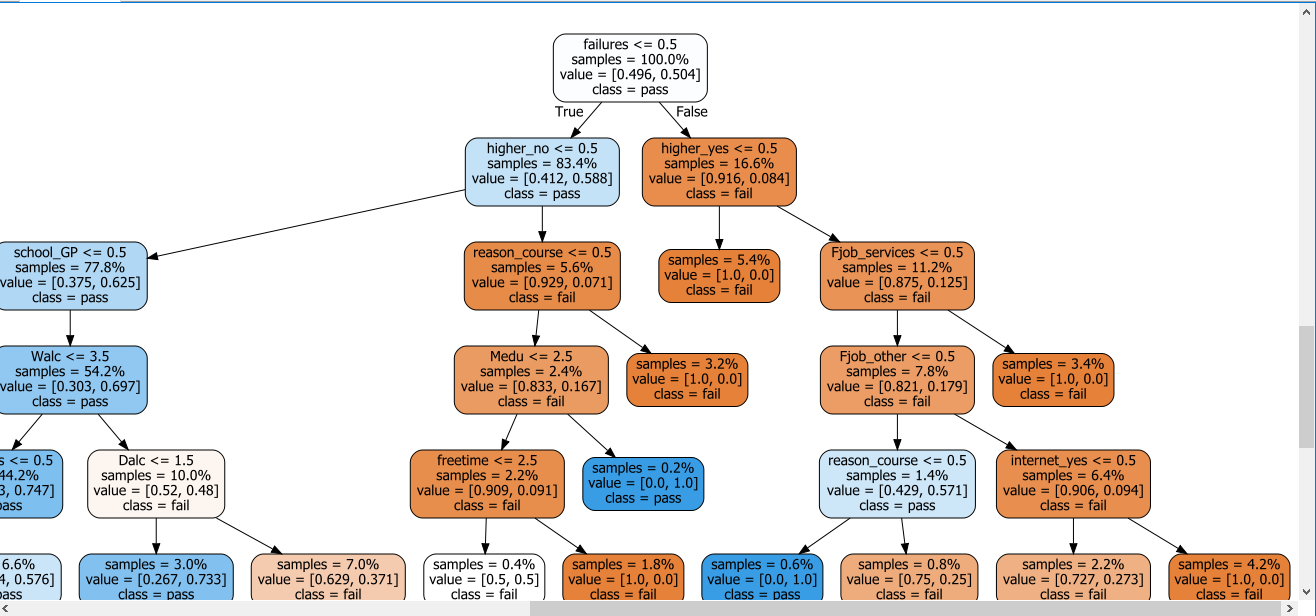
\includegraphics[width=1\textwidth]{figures/im/imCode6.png}}
		\caption{Source Code.}
		\label{enamC}
		\end{figure}
\end{itemize}

Source code 7:
		\begin{figure}[ht]
		\centerline{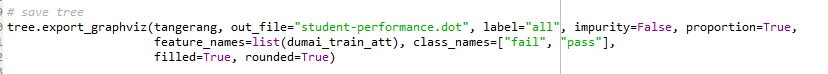
\includegraphics[width=1\textwidth]{figures/im/imQ7.png}}
		\caption{Source Code.}
		\label{tujuhQ}
		\end{figure}
\begin{itemize}
\item Source code tersebut berguna untuk mengekspor representasi visual dalam bentuk PDF atau format lainnya, seperti gambar berikut \ref{tujuhQ}
\item Berikut hasil yang di dapat dari source code berikut \ref{tujuhC}
		\begin{figure}[ht]
		\centerline{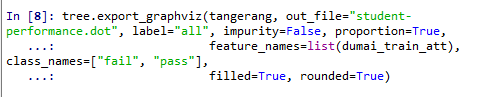
\includegraphics[width=1\textwidth]{figures/im/imCode7.png}}
		\caption{Source Code.}
		\label{tujuhC}
		\end{figure}
\end{itemize}

Source code 8:
		\begin{figure}[ht]
		\centerline{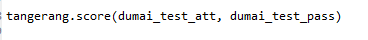
\includegraphics[width=1\textwidth]{figures/im/imQ8.png}}
		\caption{Source Code.}
		\label{delapanQ}
		\end{figure}
\begin{itemize}
\item Source code berikut \ref {delapanQ} berguna untuk memeriksa skor tree dengan menggunakan set pengujian yang telah di buat sebelumnya
\item Berikut hasil yang di dapat dari source code berikut \ref{delapanC}
		\begin{figure}[ht]
		\centerline{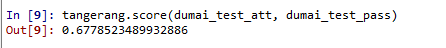
\includegraphics[width=1\textwidth]{figures/im/imCode8.png}}
		\caption{Source Code.}
		\label{delapanC}
		\end{figure}
\end{itemize}

Source code 9:
		\begin{figure}[ht]
		\centerline{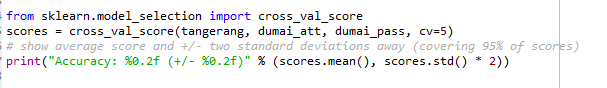
\includegraphics[width=1\textwidth]{figures/im/imQ9.png}}
		\caption{Source Code.}
		\label{sembilanQ}
		\end{figure}
\begin{itemize}
\item Pada baris pertama berguna untuk import library cross val score, seperti gambar berikut \ref{sembilanQ}
\item Baris kedua data yang telah dibuat sebelumnya akan kembali digunakan untuk memastikan rata-rata tersebut
\item Pada baris ketiga akan menampilkan hasil rata-rata dari data tersebut
\item Berikut hasil yang di dapat dari source code berikut \ref{sembilanC}
		\begin{figure}[ht]
		\centerline{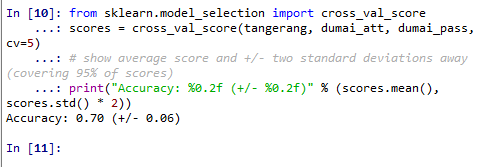
\includegraphics[width=1\textwidth]{figures/im/imCode9.png}}
		\caption{Source Code.}
		\label{sembilanC}
		\end{figure}
\end{itemize}

Source code 10:
		\begin{figure}[ht]
		\centerline{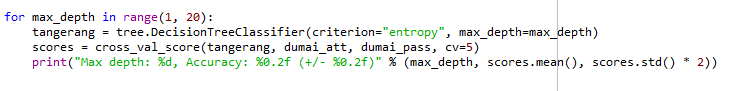
\includegraphics[width=1\textwidth]{figures/im/imQ10.png}}
		\caption{Source Code.}
		\label{sepuluhQ}
		\end{figure}
\begin{itemize}
\item Source code berikut ini berfungsi untuk melakukan pengecekan lebih dalam lagi untuk menentukan keputusan yang lebih akurat dibandingkan dengan metode sebelumnya. Pada source code tersebut melakukan validasi silang, seperti gambar berikut \ref{sepuluhQ}
\item Berikut hasil yang di dapat dari source code berikut \ref{sepuluhC}
		\begin{figure}[ht]
		\centerline{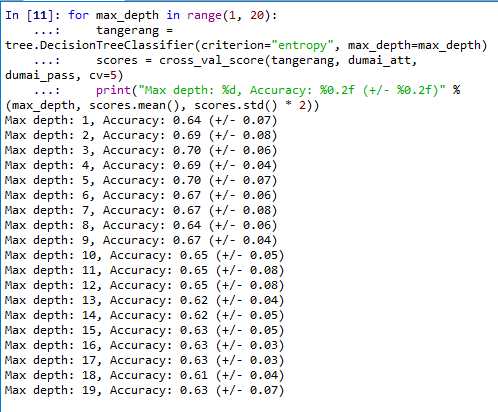
\includegraphics[width=1\textwidth]{figures/im/imCode10.png}}
		\caption{Source Code.}
		\label{sepuluhC}
		\end{figure}
\end{itemize}

Source code 11:
		\begin{figure}[ht]
		\centerline{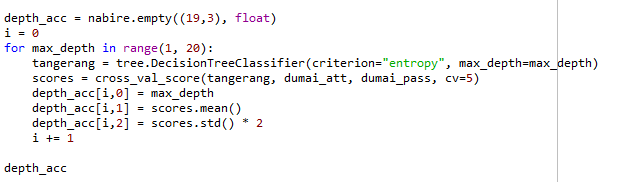
\includegraphics[width=1\textwidth]{figures/im/imQ11.png}}
		\caption{Source Code.}
		\label{sebelasQ}
		\end{figure}
\begin{itemize}
\item Source code tersebut menjelaskan bahwa untuk mendapatkan hasil keputusan yang akurat diperlukan training yang lebih banyak lagi dalam kasus ini depth acc  memiliki nilai 19 dan 3. Proses yang dilakukan sama dengan proses sebelumnya yakni dengan menggunakan decision tree dan dari data hasil data training dan data testing, seperti gambar berikut \ref{sebelasQ}
\item Berikut hasil yang di dapat dari source code berikut \ref{sebelasC}
		\begin{figure}[ht]
		\centerline{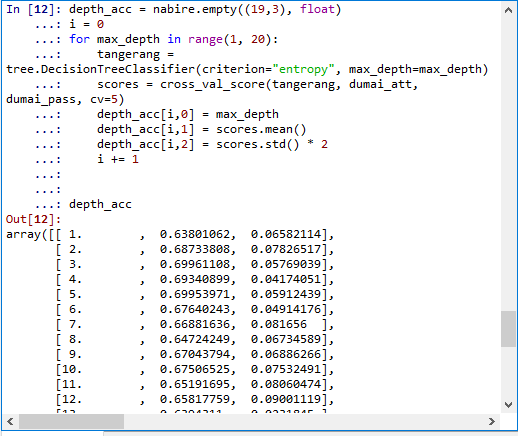
\includegraphics[width=1\textwidth]{figures/im/imCode11.png}}
		\caption{Source Code.}
		\label{sebelasC}
		\end{figure}
\end{itemize}

Source code 12:
		\begin{figure}[ht]
		\centerline{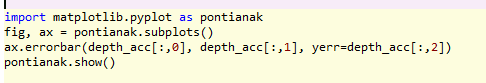
\includegraphics[width=1\textwidth]{figures/im/imQ12.png}}
		\caption{Source Code.}
		\label{duabelasQ}
		\end{figure}
\begin{itemize}
\item Pada baris pertama berguna untuk import library matplotlib.pyplot, seperti gambar berikut \ref{duabelasQ}
\item Source code tersebut berguna untuk menampilkan diagram hasil keputusan pada pelatihan-pelatihan data sebelumnya
\item Berikut hasil yang di dapat dari source code berikut \ref{duabelasC}
		\begin{figure}[ht]
		\centerline{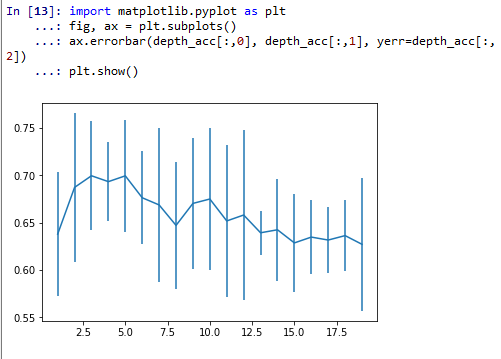
\includegraphics[width=1\textwidth]{figures/im/imCode12.png}}
		\caption{Source Code.}
		\label{duabelasC}
		\end{figure}
\end{itemize}

\subsection{Penanganan Error}
Dari percobaan yang telah dilakukan saya mengalami 2 kali error, berikut screenshot error serta penaganan yang saya dapat:
\begin{enumerate}
\item Screenshot error \ref{Error1}
		\begin{figure}[ht]
		\centerline{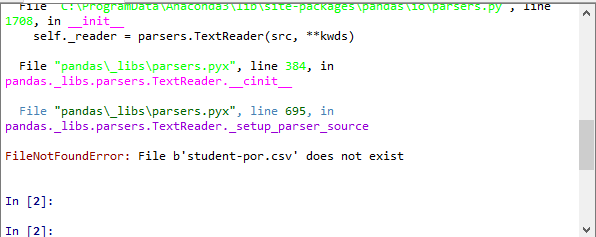
\includegraphics[width=1\textwidth]{figures/im/imError1.png}}
		\caption{Error.}
		\label{Error1}
		\end{figure}
\item Solusi dari permasalahan tersebut, kita tinggal memasukan direktori tempat file tersebut berada \ref{imResolve1}
		\begin{figure}[ht]
		\centerline{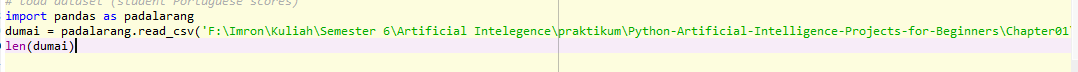
\includegraphics[width=1\textwidth]{figures/im/imResolve1.png}}
		\caption{Resolve.}
		\label{imResolve1}
		\end{figure}
\item Screenshot error \ref{Error2}
		\begin{figure}[ht]
		\centerline{\includegraphics[width=1\textwidth]{figures/im/imErrror2.png}}
		\caption{Error.}
		\label{Error2}
		\end{figure}
\item Solusi dari permasalahan tersebut, kita harus install library graphviz terlebih dahulu seperti gambar \ref{imResolve2}, berhubung saya sudah install maka gambarnya seperti itu. 
		\begin{figure}[ht]
		\centerline{\includegraphics[width=1\textwidth]{figures/im/imResolve2.png}}
		\caption{Resolve.}
		\label{imResolve2}
		\end{figure}
\item Selanjutnya setalah install library graphviz selesai, kita masukkan path graphviz tersebut kedalam environment variables seperti gambar \ref{imResolve3} agar dapat digunakan. 
		\begin{figure}[ht]
		\centerline{\includegraphics[width=1\textwidth]{figures/im/imResolve3.png}}
		\caption{Resolve.}
		\label{imResolve3}
		\end{figure}
\item Setelah itu semua selesai, maka permasalahan pun sudah ditangani.
\end{enumerate}

\section{scikit-learn}
HARI KEDUA ANDRI FAJAR SUNANDHAR 1164065

\begin{enumerate}

\item
\begin{verbatim}
	# load dataset (student Portuguese scores)
	import pandas as apel
	jeruk = apel.read_csv('E:\KAMPUS\Semester 6\Kecerdasan Buatan\modul\Python-Artificial-Intelligence-Projects-for-			 	Beginners\Chapter01\dataset\student-mat.csv', sep=';')
	len(jeruk)
\end{verbatim}

\par
Untuk mengimport atau memanggil module pandas sebagai apel. Kemudian mendefinisikan variabel "jeruk" yang akan memanggil dataset yang didapatkan dari data student-mat.csv 
\begin{figure}[ht]
\centering
\includegraphics[scale=0.5]{figures/spyder/1.png}
\caption{Loading Dataset}
\label{Spyder}
\end{figure}
\item
\begin{verbatim}
	# generate binary label (pass/fail) based on G1+G2+G3 (test grades, each 0-20 pts); threshold for passing is sum>=30
	jeruk['pass'] = jeruk.apply(lambda row: 1 if (row['G1']+row['G2']+row['G3']) >= 35 else 0, axis=1)
	jeruk = jeruk.drop(['G1', 'G2', 'G3'], axis=1)
	jeruk.head()
\end{verbatim}

\par
mendeklarasikan label pass/fail nya data berdasarkan G1+G2+G3. 
kemudian pada variabel jeruk dideklarasikan  jika baris dengan G1+G2+G3 ditambahkan, dan hasilnya sama dengan 35 maka axisnya 1. 
\begin{figure}[ht]
\centering
\includegraphics[scale=0.5]{figures/spyder/2.png}
\caption{Generate Binary Label}
\label{Spyder}
\end{figure}
\item
\begin{verbatim}
	# use one-hot encoding on categorical columns
	jeruk = apel.get_dummies(jeruk, columns=['sex', 'school', 'address', 'famsize', 'Pstatus', 'Mjob', 'Fjob', 
                               'reason', 'guardian', 'schoolsup', 'famsup', 'paid', 'activities',
                               'nursery', 'higher', 'internet', 'romantic'])
	jeruk.head()
\end{verbatim}
\par
One-hot encoding adalah proses di mana variabel kategorikal dikonversi menjadi bentuk yang dapat disediakan untuk algoritma .
\begin{figure}[ht]
\centering
\includegraphics[scale=0.5]{figures/spyder/3.png}
\caption{One-hot Encoding}
\label{Spyder}
\end{figure}
\item
\begin{verbatim}
	# shuffle rows
	jeruk = jeruk.sample(frac=1)
	# split training and testing data
	jeruk_train = jeruk[:500]
	jeruk_test = jeruk[500:]

	jeruk_train_att = jeruk_train.drop(['pass'], axis=1)
	jeruk_train_pass = jeruk_train['pass']

	jeruk_test_att = jeruk_test.drop(['pass'], axis=1)
	jeruk_test_pass = jeruk_test['pass']

	jeruk_att = jeruk.drop(['pass'], axis=1)
	jeruk_pass = jeruk['pass']

	# number of passing students in whole dataset:
	import numpy as np
	print("Passing: %d out of %d (%.2f%%)" % (np.sum(jeruk_pass), len(jeruk_pass), 100*float(np.sum(jeruk_pass)) / 	len(jeruk_pass)))
\end{verbatim}

\par
 Pada bagian tersebut, terdapat train dan test yaing digunakan untuk untuk membagi train, test dan kemudian membagi lagi train ke validasi dan test.\\
Kemudia akan mengimport module numpy sebagai np yang akan digunakan untuk mengembalikan nilai passing dari pelajar dari keseluruhan dataset dengan cara print.
\begin{figure}[ht]
\centering
\includegraphics[scale=0.5]{figures/spyder/4.png}
\caption{Shuffle Rows}
\label{Spyder}
\end{figure}
\item 
\begin{verbatim}
	# fit a decision tree
	from sklearn import tree
	semangka = tree.DecisionTreeClassifier(criterion="entropy", max_depth=5)
	semangka = semangka.fit(jeruk_train_att, jeruk_train_pass)
\end{verbatim}

\par
Dari librari scikitlearn import modul tree. Kemudian definisikan variabel semangka dengan menggunakan DecisionTreeClassifier. Kemudian pada variabel semangka terdapat Criterion , setelah itu agar DecisionTreeClassifier dapat dijalankan gunakan perintah fit. hasilnya seperti dibawah
\begin{figure}[ht]
\centering
\includegraphics[scale=0.5]{figures/spyder/5.png}
\caption{Fit Decision Tree}
\label{Spyder}
\end{figure}
\item
\begin{verbatim}
	# visualize tree
	import graphviz
	dot_data = tree.export_graphviz(semangka, out_file=None, label="all", impurity=False, proportion=True,
                                feature_names=list(jeruk_train_att), class_names=["fail", "pass"], 
                                filled=True, rounded=True)
	graph = graphviz.Source(dot_data)
	graph
\end{verbatim}

\par
Mengimport Graphviz Sehingga akan muncul gambardiagram  grafik bercabang.
\begin{figure}[ht]
\centering
\includegraphics[scale=0.5]{figures/spyder/6.png}
\caption{Fit Decision Tree}
\label{Spyder}
\end{figure}
\item
\begin{verbatim}
	# save tree
	tree.export_graphviz(semangka, out_file="student-performance.dot", label="all", impurity=False, proportion=True,
                     feature_names=list(jeruk_train_att), class_names=["fail", "pass"], 
                     filled=True, rounded=True)
\end{verbatim}

\par
tree.exportgraphviz merupakan fungsi yang menghasilkan representasi Graphviz dari decision tree.
\begin{figure}[ht]
\centering
\includegraphics[scale=0.5]{figures/spyder/7.png}
\caption{Fit Decision Tree}
\label{Spyder}
\end{figure}
\item
\begin{verbatim}
	semangka.score(jeruk_test_att, jeruk_test_pass)
\end{verbatim}

\par
Score juga disebut prediksi, Nilai atau skor yang dibuat dapat mewakili prediksi nilai masa depan, tetapi mereka juga mungkin mewakili kategori atau hasil yang mungkin. disini semangka akan memprediksi jeruk.
\begin{figure}[ht]
\centering
\includegraphics[scale=0.5]{figures/spyder/88.jpeg}
\caption{Score}
\label{Spyder}
\end{figure}
\item
\begin{verbatim}
	from sklearn.model_selection import cross_val_score
	scores = cross_val_score(semangka, jeruk_att, jeruk_pass, cv=5)
	# show average score and +/- two standard deviations away (covering 95% of scores)
	print("Accuracy: %0.2f (+/- %0.2f)" % (scores.mean(), scores.std() * 2))
\end{verbatim}

\par
 Dari sklearn.modelselection akan mengimport crossvalscore. Kemudian akan menampilkan score rata rata dan kurang lebih dua standar deviasi yang mencakup 95 persen score.
\begin{figure}[ht]
\centering
\includegraphics[scale=0.5]{figures/spyder/9.png}
\caption{Cross Val Score}
\label{Spyder}
\end{figure}
\item 
\begin{verbatim}
	for max_depth in range(1, 20):
   	 semangka = tree.DecisionTreeClassifier(criterion="entropy", max_depth=max_depth)
    	scores = cross_val_score(semangka, jeruk_att, jeruk_pass, cv=5)
    	print("Max depth: %d, Accuracy: %0.2f (+/- %0.2f)" % (max_depth, scores.mean(), scores.std() * 2))
\end{verbatim}

\par
Semangka akan mendefinisikan tree.DecissionTreeClassifier nya yang kemudian variabel semangka akan mengevaluasi score dengan validasi silang.
\begin{figure}[ht]
\centering
\includegraphics[scale=0.5]{figures/spyder/10.png}
\caption{Max Depth}
\label{Spyder}
\end{figure}
\item
\begin{verbatim}
	depth_acc = np.empty((19,3), float)
	i = 0
	for max_depth in range(1, 20):
    	semangka = tree.DecisionTreeClassifier(criterion="entropy", max_depth=max_depth)
    	scores = cross_val_score(semangka, jeruk_att, jeruk_pass, cv=5)
   	 depth_acc[i,0] = max_depth
   	 depth_acc[i,1] = scores.mean()
   	 depth_acc[i,2] = scores.std() * 2
   	 i += 1
    
	depth_acc

\end{verbatim}

\par
Dengan 19 sebagai bentuk array kosong, 3 sebagai output data-type dan float urutan kolom-utama (gaya Fortran) dalam memori. variabel semangka yang akan melakukan split score dan nangka akan mengvalidasi score secara silang. 
\begin{figure}[ht]
\centering
\includegraphics[scale=0.5]{figures/spyder/11.png}
\caption{Depth in Range}
\label{Spyder}
\end{figure}
\item 
\begin{verbatim}
	import matplotlib.pyplot as plt
	fig, ax = plt.subplots()
	ax.errorbar(depth_acc[:,0], depth_acc[:,1], yerr=depth_acc[:,2])
	plt.show()
\end{verbatim}

\par
Mengimpor librari dari matplotlib yaitu pylot sebagai plt\\
fig dan ax menggunakan subplots untuk membuat gambar .\\
ax.errorbar akan membuat error bar
\\
\\
\\
\begin{figure}[ht]
\centering
\includegraphics[scale=0.5]{figures/spyder/12.png}
\caption{Matplotlib}
\label{Spyder}
\end{figure}
\end{enumerate}

\section{Penanganan Error}
Hari Kedua Andri fajar Sunandhar 1164065
\subsection{Error Graphviz}
\begin{enumerate}
	\item
error yang didapatkan saat menjalankan Graphviz
\begin{figure}[ht]
\centering
\includegraphics[scale=0.5]{figures/spyder/20.png}
\caption{Error Graphviz}
\label{Error}
\end{figure}
	\item
Kode erornya adalah ModuleNotFoundError. Eror ini terjadi karena module named Graphviz nya tidak ada.
	\item
Solusi yang bisa dilakukan untuk mengatasi eror tersebut adalah sebagai berikut : \\
\begin{itemize}
\item
buka CMD kemudian perintah pip install graphviz
\begin{figure}[ht]
\centering
\includegraphics[scale=0.5]{figures/spyder/21.png}
\caption{install Graphviz}
\label{solusi}
\end{figure}
\item
masukan perintah conda install pip, untuk solving environment
\begin{figure}[ht]
\centering
\includegraphics[scale=0.5]{figures/spyder/22.png}
\caption{Solving Environment}
\label{solusi}
\end{figure}
\item
selanjutnya masukan perintah conda install python-graphviz , untuk menambahkan package python-graphviz pada conda
\begin{figure}[ht]
\centering
\includegraphics[scale=0.5]{figures/spyder/23.png}
\caption{Evaluasi Eror}
\label{Eror}
\end{figure}
\end{itemize}
\end{enumerate}

